\section{Methods}

\subsection{Architecture}\label{methods:Architecture}
    In Deep-Learning based compression, an encoder NN embeds data in a latent space, where it is losslessly encoded and transmitted. The decoder NN decompresses the latent space and returns to the input domain.

    \begin{figure}[H]
        \centering
        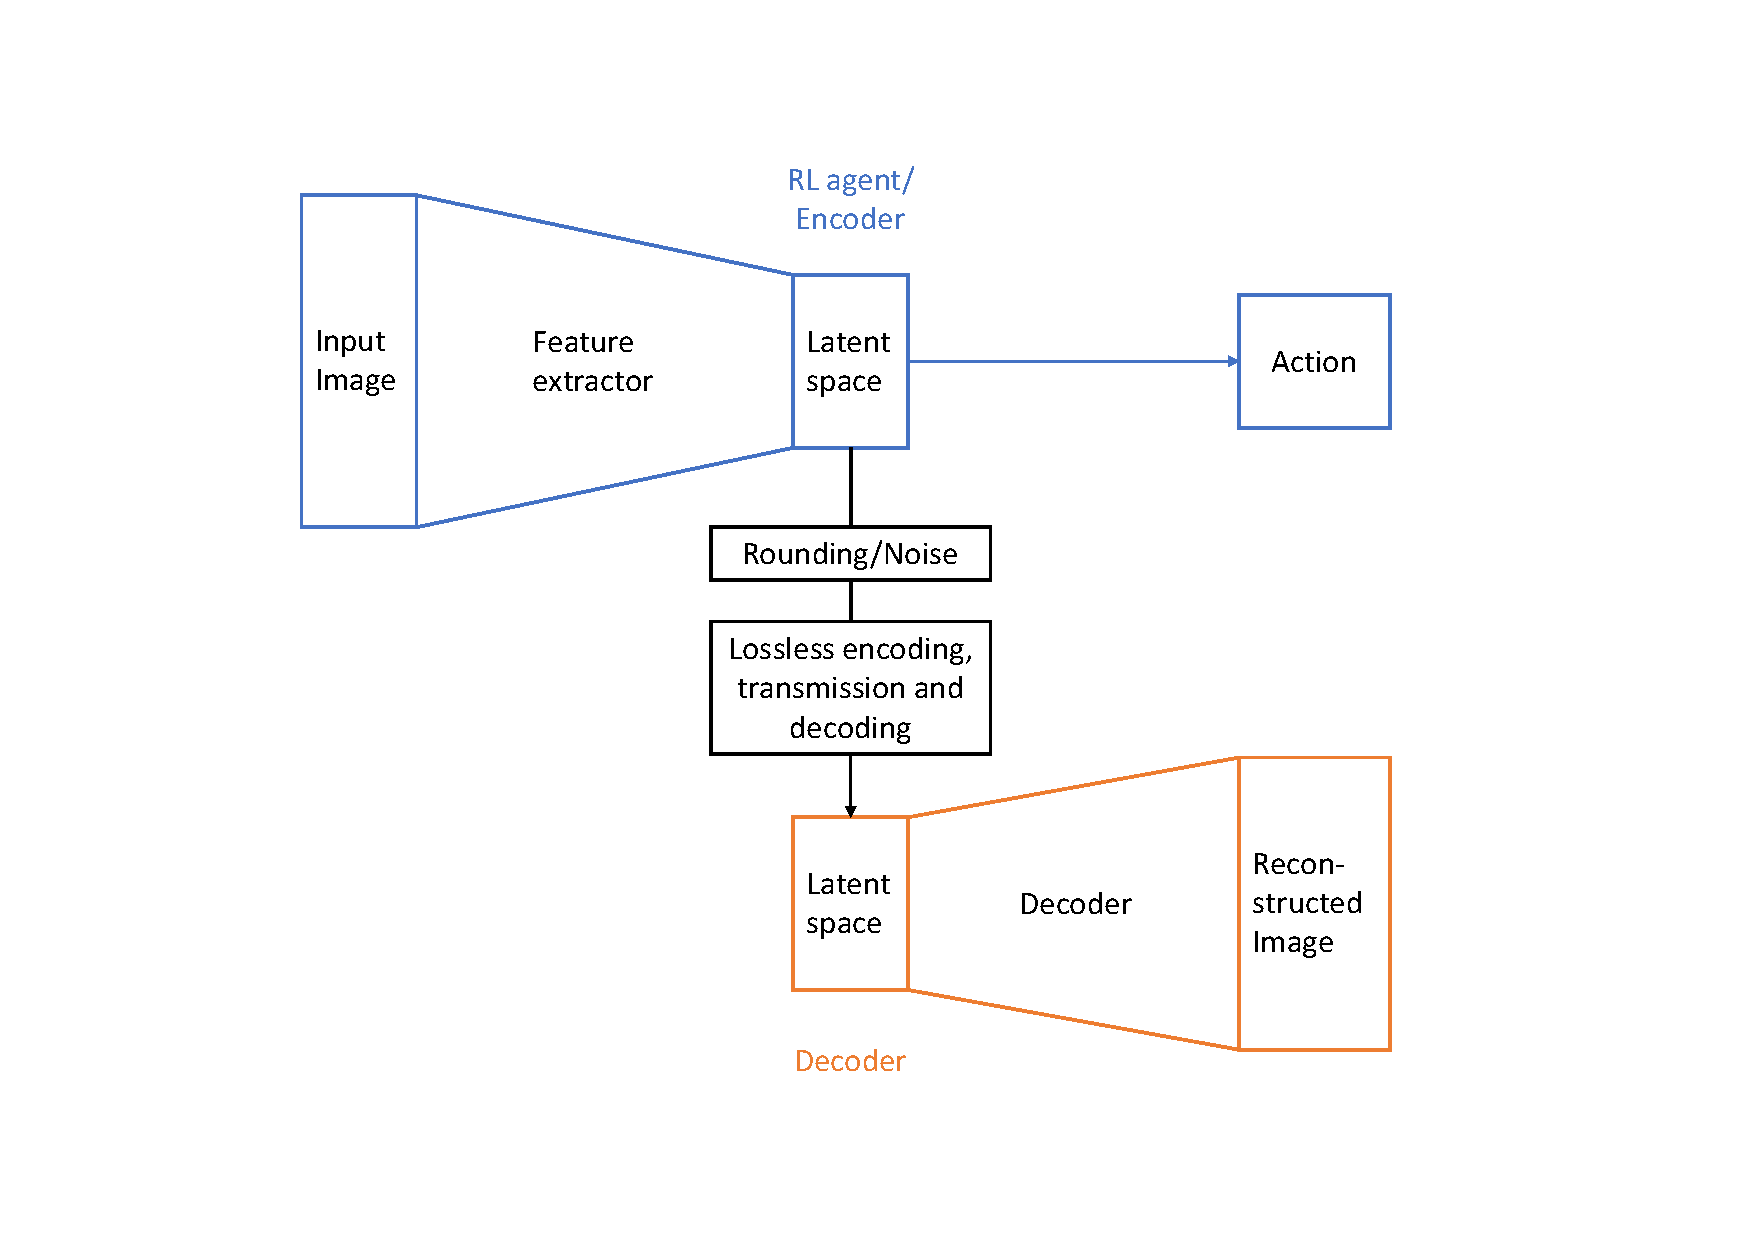
\includegraphics[width=\linewidth]{images/architecture.pdf}
        \caption{Overall architecture}
        \label{fig:Architecture}
    \end{figure}

    In our approach, a RL agent acts as the first
    NN. The agent contains a feature extractor, which
    extracts information to determine
    the action. Ideally, this content should also be important
    for reconstruction. Then the latent space is losslessly encoded and
    transmitted with an algorithm of choice, such as ANS (for training this
    step is unnecessary as the latents will be losslessly decompressed). After decoding, the latents they are passed through a normal upsampling NN.
    Figure \ref{fig:Architecture} shows an overview of the architecture.

\subsection{Theory}
    Lossy compression balances a low bitrate and a low distortion.
    This section describes how these objectives apply to our project.

    \subsubsection{Bitrate}
        Determining algorithm bitrate requires observing the encoding
        process, where the input image is mapped to the
        latent space, see \ref{methods:Architecture}. This decreases the
        image bitrate if the latent entropy is lower than the image entropy and a sufficient encoding distribution for latent transmission is chosen. If the latent
        space distribution of $z$ is given by $Q_\theta(Z=z \vert x)$ where $\theta$
        parametrizes the distribution and $P(Z=z)$ is used to encode the latents for transmission, the bitrate is given by the cross entropy
        \begin{equation}\label{eq:BitRate}
            \mathbb{E}_{z \sim Q_\theta(Z=z \vert x)}[log(P(Z=z))]
        \end{equation}
        In addition, $Q=P$ will give the perfect encoding distribution. Hence, the
        entropy is a lower bound on the cross-entropy.

        Because NNs have real valued outputs, $Q_\theta(Z=z
        \vert x)$ is a continuous PDF, resulting in a high bit rate. Therefore, one
        approach is to round the latents \cite{DBLP:journals/corr/BalleLS16a}. This reduces $Q$ to a discrete
        probability distribution, which reduces the cross entropy. However, rounding
        is undesirable during training, since its gradient is 0 nearly everywhere. Therefore, we replace
        rounding during training with adding uniform noise $u$, see also
        figure \ref{fig:Architecture}. This shifts the values
        similarly to rounding, but is differentiable.

        Another effect of adding uniform noise is that we can reparametrize equation
        \ref{eq:BitRate} and take the expectation over the uniform noise:
        \begin{equation}
            \mathbb{E}_{u \sim U[-\epsilon, \epsilon]}[log(P(Z=\hat{z} + u))]
        \end{equation}
        where $\hat{z}$ is the mean of $Q_\theta(Z=z \vert x)$. \newline

        % (To be more precise: We start with a continuous pdf. Rounding creates a
        % bunch of delta pulses which are nondifferentiable. However we can
        % approximate the continuous pdf by adding uniform noise to the new discrete
        % pdf. Therefore we can also just add noise instead of round?)


        % In turn, this means that the encoding network shouldn't encode information
        % in small differences. One approach to achieve this behaviours is to add
        % noise to the latent values, which forces the RL-agent to get more robust to
        % noise.

        % [TODO: this part is just disregared in balle]
        The encoding distribution $P$ is naively chosen as Normal. The
        mean can be chosen arbitrarily given a powerful enough transformation, so it is
        set to 0 for simplicity. The variance is learned during the training process.

    \subsubsection{Distortion}\label{sub:Distortion}
        Bitrate decrease is often traded for distortion increase.
        Therefore, we need a performance measure to evaluate reconstructed image distortion $\hat{x}$. A traditional metric is the Mean Squared Error (MSE),
        \begin{equation}\label{equ:L2}
            \mathbb{E}_{x, \hat{x}}[\sum_{i,j} (x_{ij} - \hat{x}_{ij})^2]
        \end{equation}
        Early experimentation (see section 4.1) found that some task-important details, specifically ball location, were omitted as they accumulated little MSE penalty; attempting to
        recover these aspects, we devised a second loss scheme, referred to as
        latent loss. The motivation was to reward the decoder for reconstructing the
        image such that the same features would be extracted, resulting in
        important aspect preservation. For this loss, we passed the
        reconstructed image through the feature extractor and evaluated the MSE
        between the original and reconstructed latent space.


        % If humans look at images however, they often just care about specific types
        % of distortion. A slightly lower brightness for example wouldn't matter for
        % most images, but probably a different colour or more generally they care
        % more about semantic distortion that would give them a different
        % interpretation and representation of the image. MSE however gives these
        % distortions all the same values.

        % As the RL-Agent is used to encode the data and therefore should extract the
        % relevant features, it seems reasonable to let the agent also judge the
        % reconstruction. Therefore, a second approach will be to compare not the
        % original image and the reconstuction, but rather the agents representation
        % of the images to measure similarity. In practive, this means passing both
        % images through the feature extractor and measuring the L2 distance in latent
        % space.


        % \subsection{Decoder loss}\label{sub:Decoder_Loss}
        %     For our decoder, we tried several loss functions. The simplest version was
        %     the MSE between the original and reconstructed images. \\
        %     In early experimentation (see section 4.1), we found that some details which
        %     may be considered important to the task, specifically the location of the
        %     ball, were omitted as they accumulated little MSE penalty; in an attempt to
        %     recover these aspects, we devised a second loss scheme, which we refer to as
        %     latent loss. The motivation was to reward the decoder for reconstructing the
        %     image in such a way that the same features would be extracted, resulting in
        %     preserving the most important aspects. For this loss, we passed the
        %     reconstructed image through the feature extractor and evaluated the MSE
        %     between the original latent space and the reconstructed latent space.





    % \subsection{Objective function from view of variational inference}
    %     In Lossy image compression, the objective function is given by the ELBO:
    %     \begin{align}
    %         & \mathbb{E}_{z \sim Q(Z= z)}[log P(X, Z= z) - log Q(Z = z)]\\
    %         & = \mathbb{E}_{z \sim Q(Z= z)}[log P(X \vert Z= z) - log \frac{Q(Z = z)}{P(Z = z)}]\\
    %         & = \mathbb{E}_{z \sim Q(Z= z)}[log P(X \vert Z= z)] - D_{KL}[Q(Z = z)\Vert P(Z = z)]\\
    %     \end{align}

    %     Problem is, that we cannot differenciate by q since expectation is over q,
    %     so just fix q by uniform distribution, and do reparametrization trick

    %     now entropy of q becomes fixed so we can remove from optimization, just need
    %     to care about $E_U[P(Z + U)]$

    %     just need to choose encoding distribution, choose naively as normal with
    %     mean 0 and learned variance since needs to be flexible.

    %     for likelihood, choose normal (leads to MSE) and fix variance

\subsection{Training}
    \subsubsection{Process}
        RL-agents normally train with a specific loss function, which will be
        abstracted by $Loss_{RL}$. As the RL-agent acts as the encoder, it
        is responsible for the bitrate. Therefore we add the loss from
        \ref{eq:BitRate} to the standard RL loss:
        \begin{equation}\label{eq:RL_Training_Loss}
            \mathbb{E}_{x}[Loss_{RL}(x) + \alpha\cdot \mathbb{E}_{u \sim U[-\epsilon, \epsilon]}[log(P(Z=\hat{z} + u))]]
        \end{equation} where $\alpha \in \mathbb{R}$ is chosen to balance the two terms.
        Both expectations will be approximated by empirical means over the training
        data. As the RL-agent is independent of the decoder, we can also train it
        separately first.

        After training the RL-agent, we fix its values. Therefore, at this point
        the encoding to the latents is fixed. Now the decoder is trained. For the decoder, we use the Loss
        schemes given in section \ref{sub:Distortion}.


    \subsubsection{Adaptive alpha (omitted)}\label{sub:Adaptive_Alpha}
        During training, an issue arose in choosing $\alpha$ (see Experiments and
        Evaluation) which we believe was caused by the RL reward: the agent behaves
        randomly in early iterations and earns little reward, but improves
        drastically once learning starts. Therefore, choosing $\alpha$ too large
        prevents the agent from ever learning to complete the task, while choosing
        $\alpha$ too small allows the agent to ignore the cross entropy loss during action
        fine-tuning. We tried to resolve this with a non-static $\alpha$: as
        the reward grows, the relative importance of the two terms should stay
        approximately the same. We designed several adaptation schemes (others can be
        found in Future Work), but the general chosen algorithm was to update $\alpha$
        each time the ratio threshold was violated. We implemented this by
        \begin{equation}
            \alpha = \alpha \cdot 10 \cdot e^{-i / 1000}
        \end{equation}
        where $i$ is the number of iterations. Multiplying by the negative iterations
        ensures that $\alpha$ changes most drastically at the beginning, but
        converges over time.